\section{Trazado de la ruta}
Para el desarrollo del presente proyecto, se ha realizado el trazado preliminar de la línea de transmisión eléctrica asociada a la nueva subestación Huila 230 kV, utilizando la herramienta Google Earth. Esta plataforma permitió identificar de manera georreferenciada el punto exacto de ubicación de la subestación y definir visualmente el recorrido óptimo de la línea, considerando los criterios ya mencionados. \\
Apoyandonos de la herramienta de Google Earth.


    \begin{figure}[h!] % 'h' coloca la figura aquí
        \hfill % Espacio horizontal entre las subfiguras
        \begin{subfigure}{0.5\textwidth}
            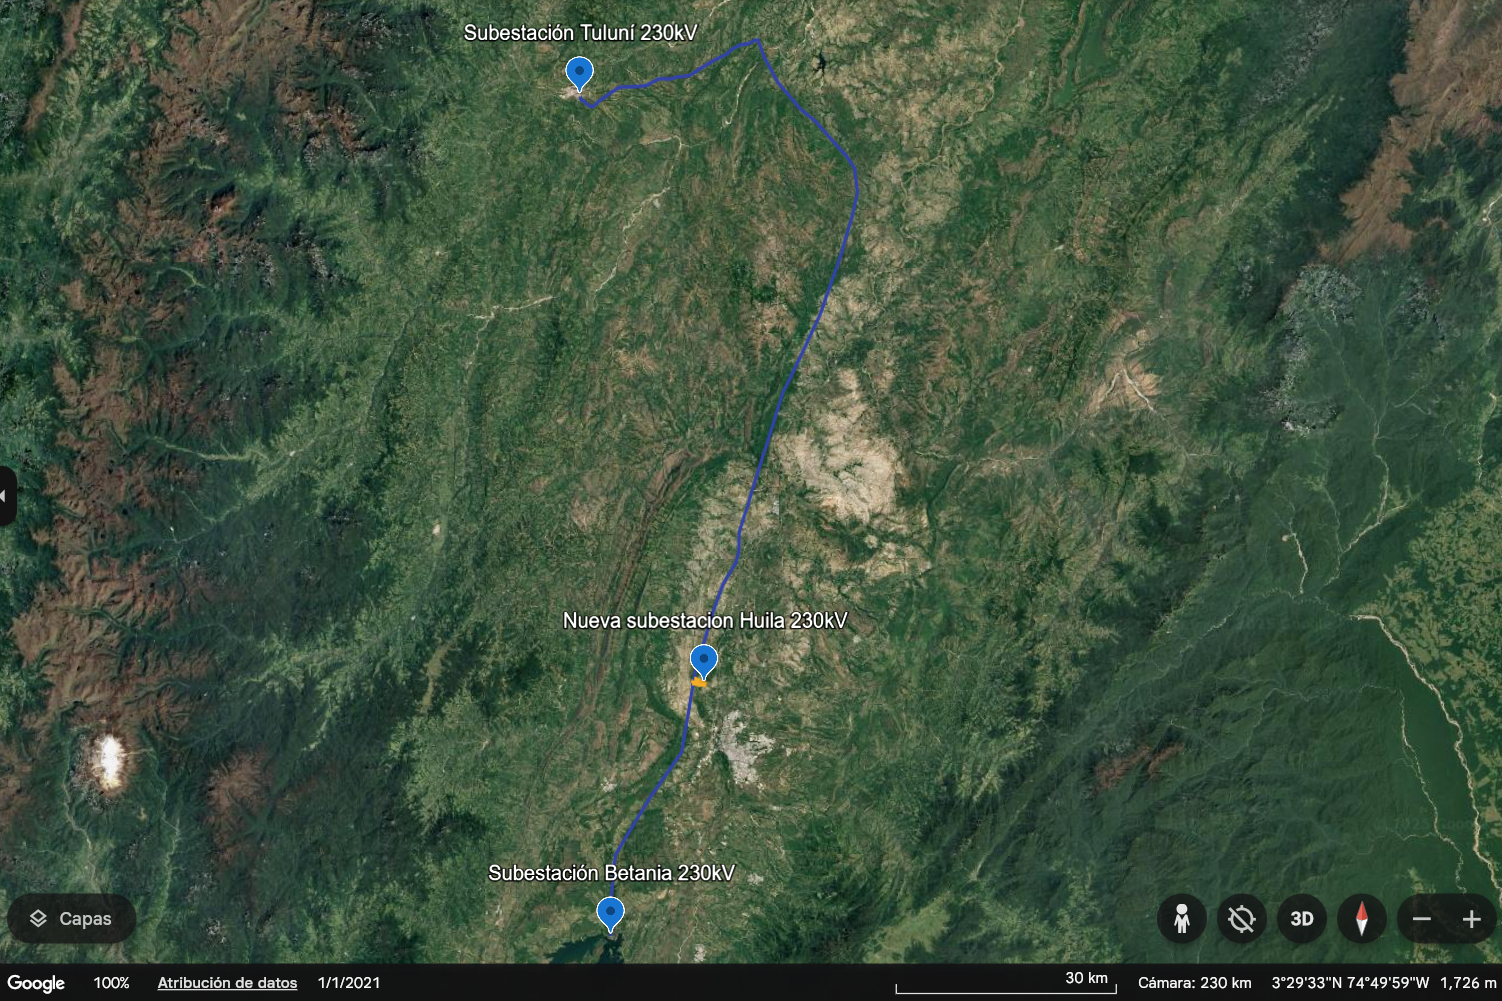
\includegraphics[width=1\textwidth]{1mer avance foticos/Huila 230kV - Google Earth - sin mirolindo.png}
            \caption{Nueva subestación huila conectada a la subestación Tuluní y Betania.} % Título de la figura
            \label{fig:sin mirolindo} % Etiqueta para referencias
        \end{subfigure}
        \begin{subfigure}{0.5\textwidth}
            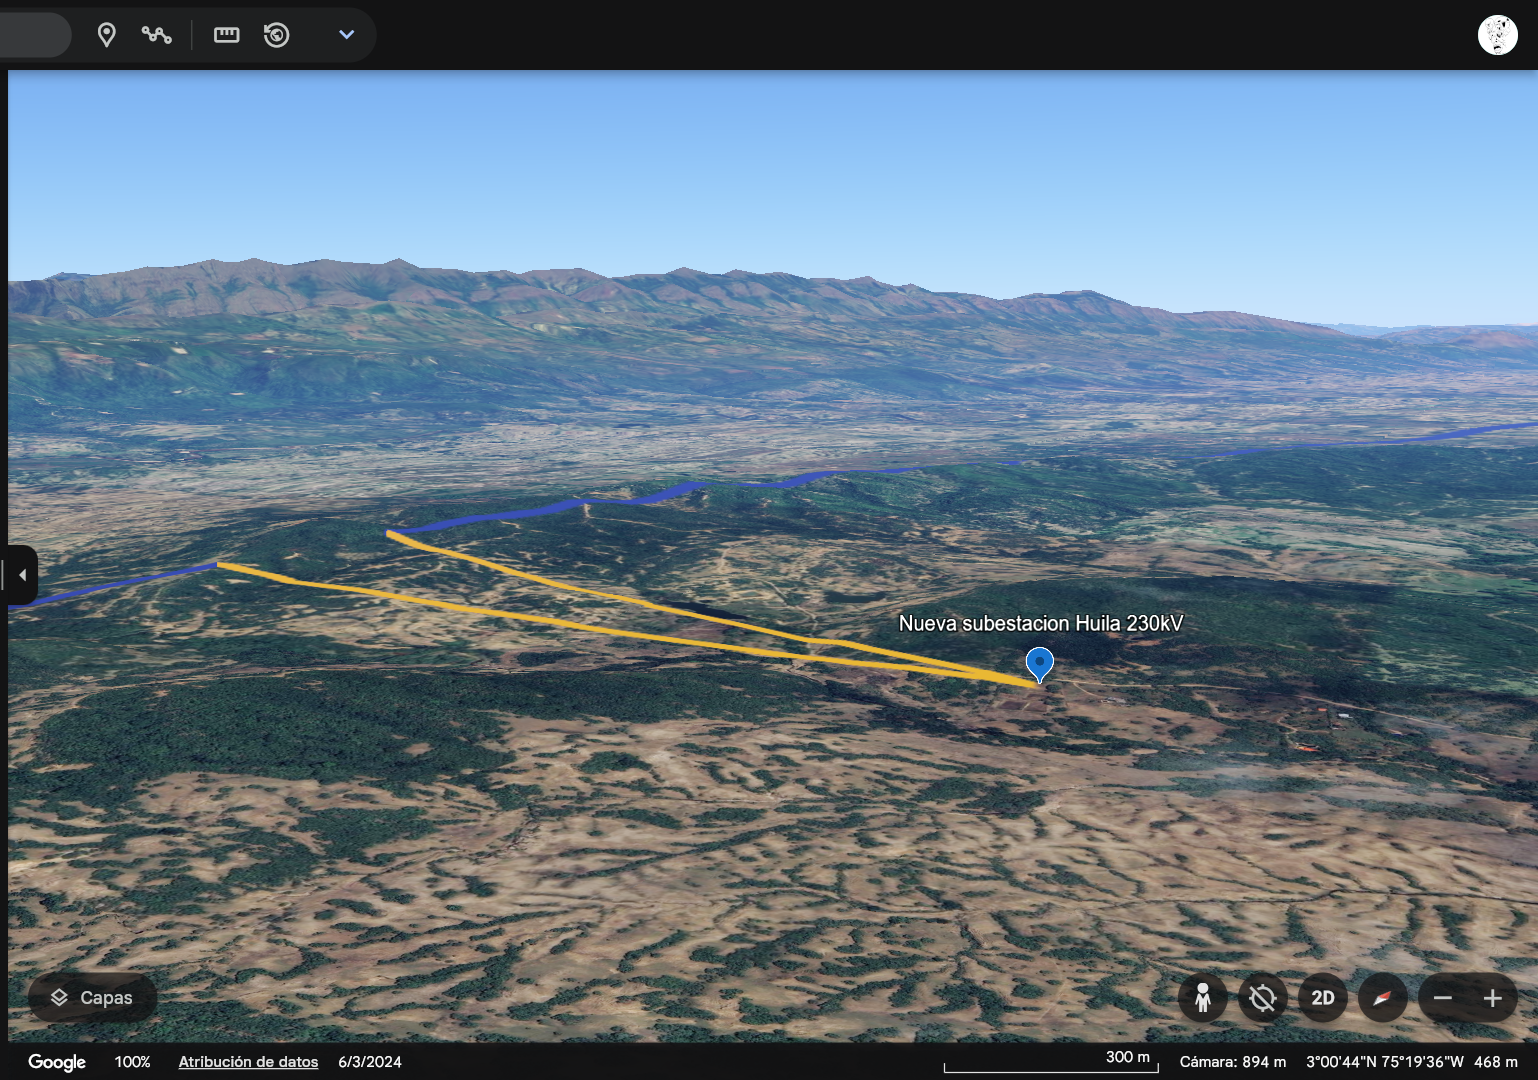
\includegraphics[width=1\textwidth]{1mer avance foticos/Huila 230kV - Google Earth - nueva acercada.png}
            \caption{Acercamiento a la nueva subestación huila conectada a la subestación Tuluní, Betania y Mirolindo.} % Título de la figura
            \label{fig:nueva acercada} % Etiqueta para referencias
        \end{subfigure}
    \end{figure}

    \begin{figure}[h!] % 'h' coloca la figura aquí
        \begin{subfigure}{0.5\textwidth}
            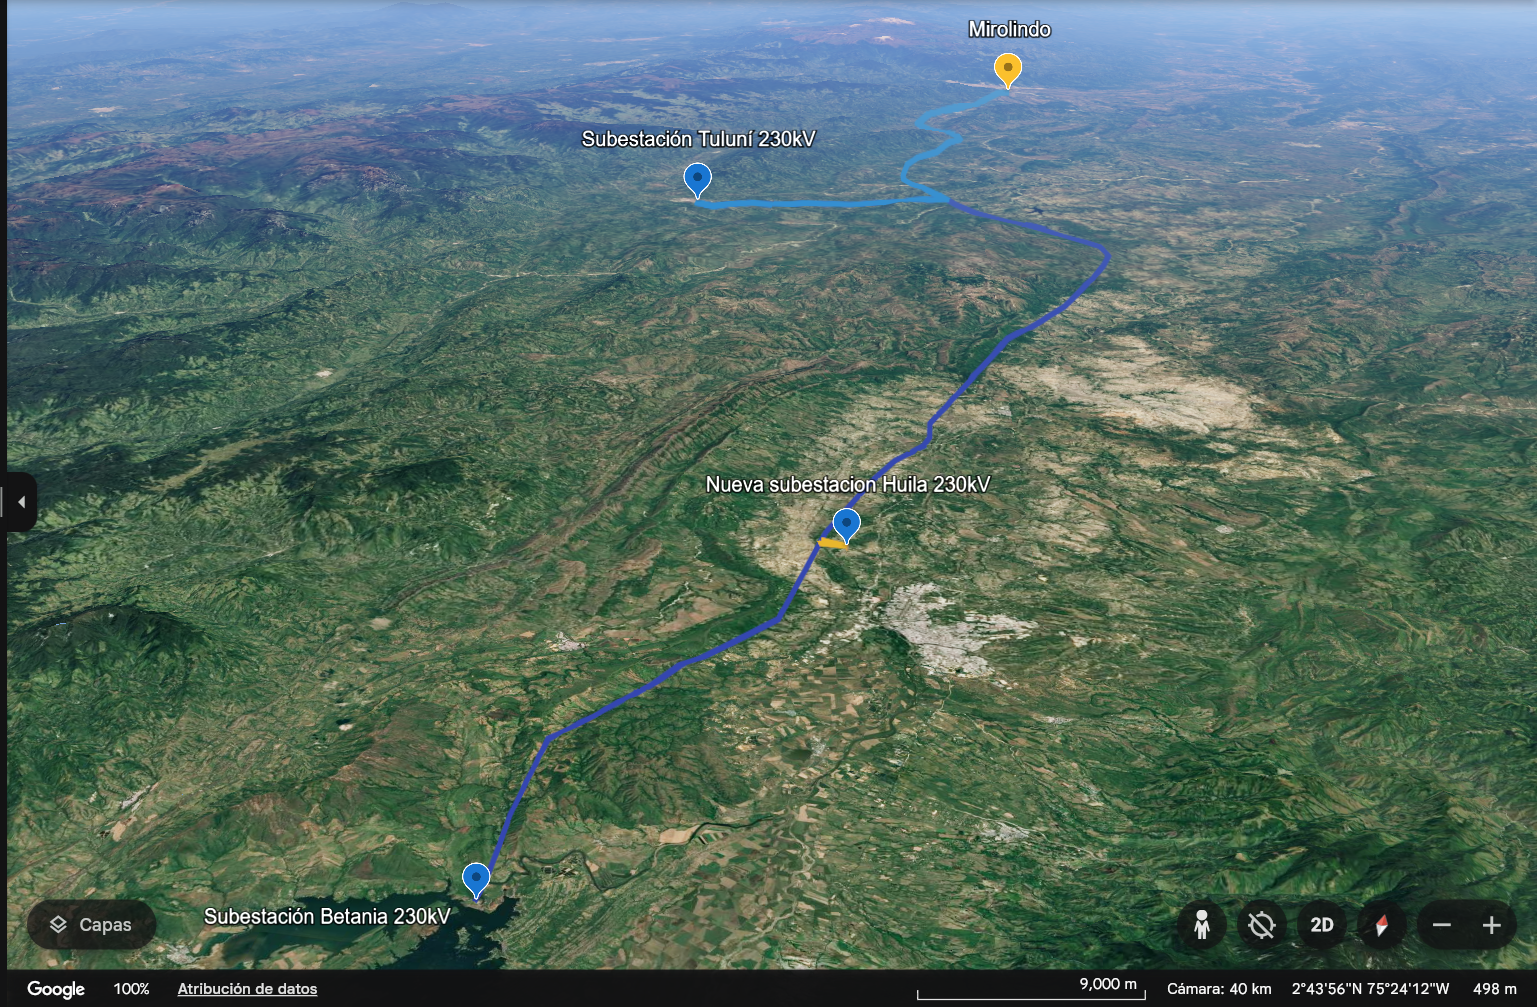
\includegraphics[width=1\textwidth]{1mer avance foticos/Huila 230kV - Google Earth - completo inclinado.png}
            \caption{Nueva subestación huila conectada a Betania con Mirolindo y conectada con Betania con Tuluní.} % Título de la figura
            \label{fig:todo angulo} % Etiqueta para referencias
        \end{subfigure}
        \hfill % Espacio horizontal entre las subfiguras
        \begin{subfigure}{0.5\textwidth}
            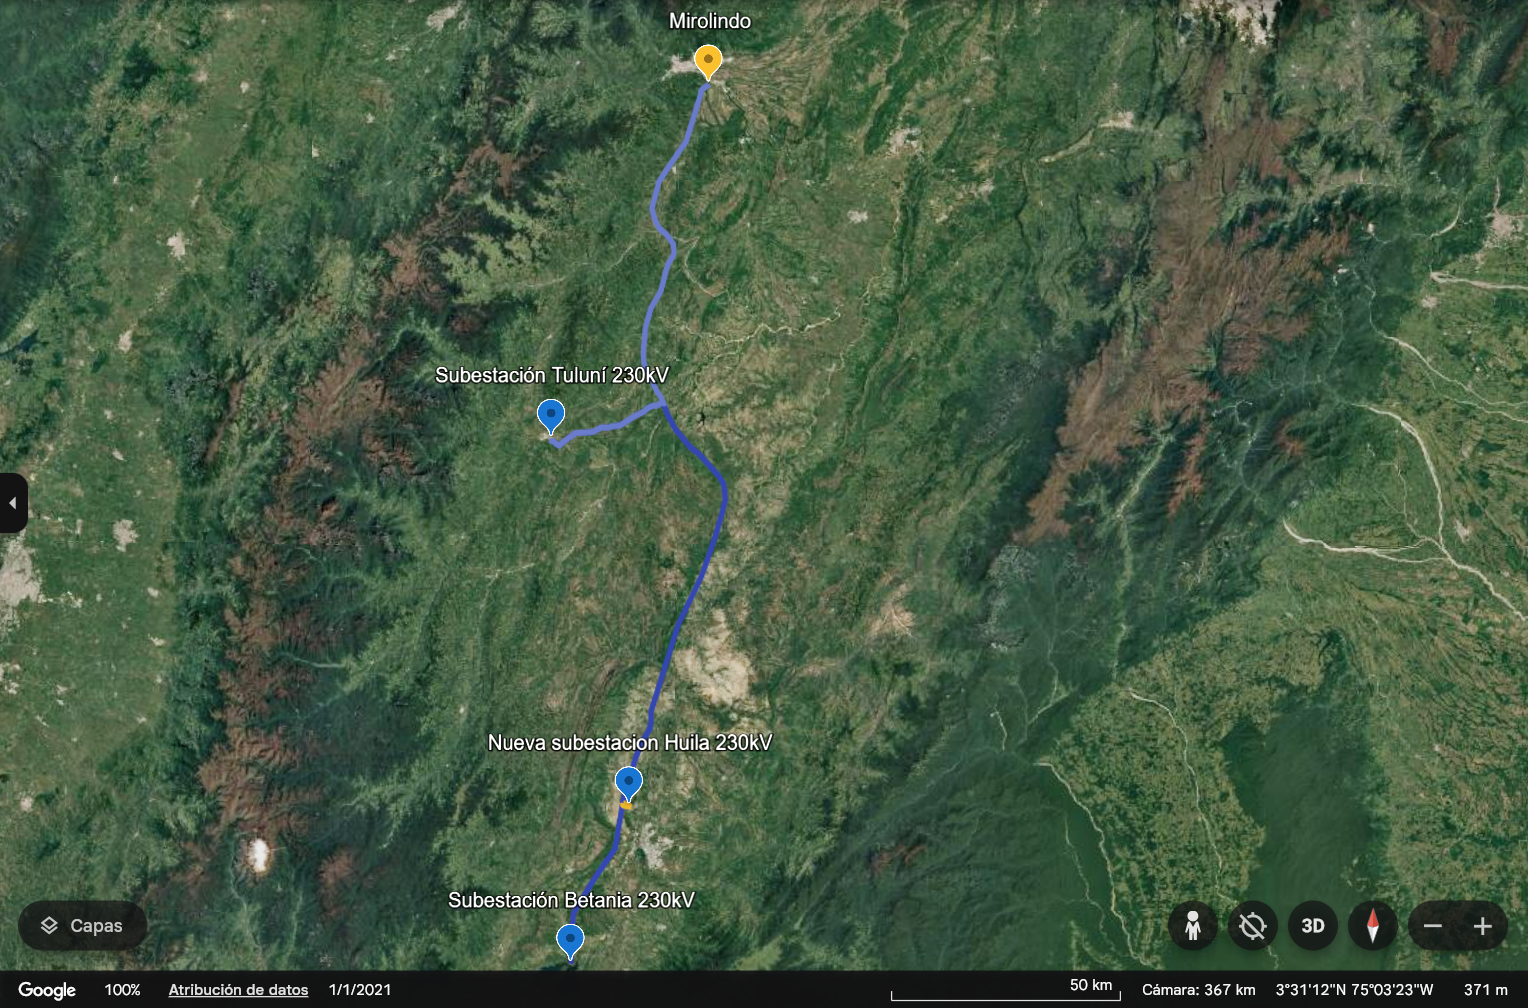
\includegraphics[width=1\textwidth]{1mer avance foticos/Huila 230kV - Google Earth - completo.png}
            \caption{Nueva subestación huila conectada a las lineas asociadas.} % Título de la figura
            \label{fig:todo} % Etiqueta para referencias
        \end{subfigure}
    \end{figure}

    \newpage